% This is text associated with the open textbook "Open Electromagnetics"
% See immediately below for author, date
% This work is licensed under the Creative Commons Attribution-ShareAlike 4.0 International License. (CC BY-SA 4.0) 
% To view a copy of the license, visit http://creativecommons.org/licenses/by-sa/4.0/

%ORB TITLE Radiation from an Electrically-Short Dipole
%ORB AUTHOR 0        # S.W. Ellingson, Virginia Tech (ellingson@vt.edu)
%ORB DATE 20191128   # yyyymmdd
%ORB ABSTRACT 

\label{m0198_Radiation_from_an_Electrically-Short_Dipole} % <-- Must match name of this file and module directory name.  Don't mess with this!
\index{antenna!electrically-short dipole (ESD)|(}
\index{electrically-short dipole|see{antenna}}

The simplest distribution of radiating current that is encountered in common practice is the electrically-short dipole (ESD).
This current distribution is shown in Figure~\ref{m0198_fESD}.
%
\begin{figure}[b!] % <--- "[b!]" for first figure in section *only*; delete for 2nd and subsequent figures
\begin{center}
\pdftooltip{{  % note double braces
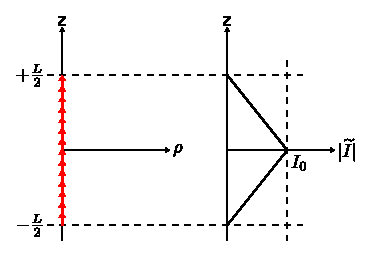
\includegraphics[width=3in]{modules/m0198_fESD.eps} 
% https://commons.wikimedia.org/wiki/File:Current_distribution_of_the_esd.svg
}}{Two coordinate systems. On the left, a vertical z-axis and a horizontal axis, small rho. On the right, a vertical z-axis and a horizontal axis absolute value of capital I tilde.  On the left graph short arrows run the length of the z-axis from negative capital L over 2 to positive capital L over 2. On the right graph, a vector from the positive z axis at capital L over 2 connects to the horizontal axis at capital I subscript 0. A second vector starting at she negative z axis at negative capital L over 2  connects to the horizontal axis at capital I subscript 0.}
\end{center}
\centerline{\scriptsize 
\copyright~\hyperref[m0198_fESD_Credit]{C.\ Wang} 
\href{https://creativecommons.org/licenses/by-sa/4.0/}{CC BY-SA 4.0} 
} % \centerline  
\caption{
\label{m0198_fESD}
Current distribution of the electrically-short dipole (ESD).
}
\end{figure}
%
The two characteristics that define the ESD are (1) the current is aligned along a straight line, and (2) the length $L$ of the line is much less than one-half of a wavelength; i.e.,  $L\ll\lambda/2$.
The latter characteristic is what we mean by ``electrically-short.''\footnote{A potential source of confusion is that the \emph{Hertzian dipole} 
\index{Hertzian dipole}
is also a ``dipole'' which is ``electrically-short.''  The distinction is that the current comprising a Hertzian dipole is \emph{constant} over its length.  This condition is rarely and only approximately seen in practice, whereas the triangular magnitude distribution is a relatively good approximation to a broad class of commonly-encountered electrically-short wire antennas.  Thus, the term ``electrically-short dipole,'' as used in this book, refers to the triangular distribution unless noted otherwise.}

The current distribution of an ESD is approximately triangular in magnitude, and approximately constant in phase. 
How do we know this?
First, note that distributions of current cannot change in a complex or rapid way over such distances which are much less than a wavelength.
If this is not immediately apparent, recall the behavior of transmission lines:  The current standing wave on a transmission line exhibits a period of $\lambda/2$, regardless the source or termination.
For the ESD, $L\ll\lambda/2$ and so we expect an even simpler variation.
Also, we know that the current at the ends of the dipole must be zero, simply because the dipole ends there.
These considerations imply that the current distribution of the ESD is well-approximated as triangular in magnitude.\footnote{A more rigorous analysis leading to the same conclusion is possible, but is beyond the scope of this book.}
Expressed mathematically:
%
\begin{equation}
\widetilde{I}(z) \approx I_0 \left(1-\frac{2}{L}\left|z\right|\right) 
\end{equation}
%
where $I_0$ (SI base units of A) is a complex-valued constant indicating the maximum current magnitude and phase.

There are two approaches that we might consider in order to find the electric field radiated by an ESD.
The first approach is to calculate the magnetic vector potential $\widetilde{\bf A}$ by integration over the current distribution, calculate $\widetilde{\bf H}=(1/\mu)\nabla\times\widetilde{\bf A}$, and finally calculate $\widetilde{\bf E}$ from $\widetilde{\bf H}$ using Ampere's law.
\index{Ampere's law!general form}
We shall employ a simpler approach, shown in Figure~\ref{m0198_fESDHD}.
%
\begin{figure} % <--- "[b!]" for first figure in section *only*; delete for 2nd and subsequent figures
\begin{center}
\pdftooltip{{  % note double braces
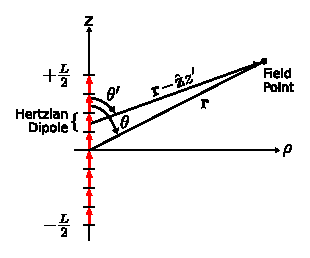
\includegraphics[width=2.5in]{modules/m0198_fESDHD.eps} 
% https://commons.wikimedia.org/wiki/File:Esd_approximated_as_a_large_number_of_hertzian_dipoles.svg
}}{A rho-z coordinate system. Small arrows run the length of the z axis from a distance negative capital L over 2 to positive capital L over 2. A single arrow is labeled Hertzian Dipole. Vector small r goes from the origin to field point in rho-z axis at an angle theta from the positive z axis. A second vector originates 1.5 arrows lengths to the field point forms an angle theta prime with the z axis. Its length is boldface small r minus boldface z hat times z. The angle vector small r makes with the z axis is theta.}
\end{center}
\centerline{\scriptsize 
\copyright~\hyperref[m0198_fESDHD_Credit]{C.\ Wang} 
\href{https://creativecommons.org/licenses/by-sa/4.0/}{CC BY-SA 4.0} 
} % \centerline 
\caption{
\label{m0198_fESDHD}
Current distribution of the electrically-short dipole (ESD) approximated as a large number of Hertzian dipoles.
}
\end{figure}
%
Imagine the ESD as a collection of many shorter segments of current that radiate independently.
The total field is then the sum of these short segments.
Because these segments are very short relative to the length of the dipole as well as being short relative to a wavelength, we may approximate the current over each segment as approximately constant. 
In other words, we may interpret each of these segments as being, to a good approximation, a Hertzian dipole.
\index{Hertzian dipole}

The advantage of this approach is that we already have a solution for each of the segments.
In Section~\ref{m0197_Radiation_from_a_Hertzian_Dipole}, it is shown that a $\hat{\bf z}$-directed Hertzian dipole at the origin radiates the electric field
%
\begin{equation}
\widetilde{\bf E}({\bf r}) \approx \hat{\bf \theta} j\eta \frac{\widetilde{I}\cdot\beta \Delta l}{4\pi}~\left(\sin\theta\right) \frac{e^{-j\beta r}}{r} 
\end{equation}
%
where $\widetilde{I}$ and $\Delta l$ may be interpreted as the current and length of the dipole, respectively.
In this expression, $\eta$ is the wave impedance of medium in which the dipole radiates (e.g., $\approx 377~\Omega$ for free space), and we have presumed lossless media such that the attenuation constant $\alpha\approx 0$ and the phase propagation constant $\beta=2\pi/\lambda$.   
This expression also assumes field points far from the dipole; specifically, distances $r$ that are much greater than $\lambda$.
Repurposing this expression for the present problem, the segment at the origin radiates the electric field:
%
\begin{equation}
\widetilde{\bf E}({\bf r};z'=0) \approx \hat{\bf \theta} j\eta \frac{I_0\cdot\beta \Delta l}{4\pi}~\left(\sin\theta\right) \frac{e^{-j\beta r}}{r} 
\end{equation}
%
where the notation $z'=0$ indicates the Hertzian dipole is located at the origin.
Letting the length $\Delta l$ of this segment shrink to differential length $dz'$, we may describe the contribution of this segment to the field radiated by the ESD as follows:
%
\begin{equation}
d\widetilde{\bf E}({\bf r};z'=0) \approx \hat{\bf \theta} j\eta \frac{I_0\cdot\beta dz'}{4\pi}~\left(\sin\theta\right) \frac{e^{-j\beta r}}{r} 
\end{equation}
% 
Using this approach, the electric field radiated by \emph{any} segment can be written:
%
\begin{equation}
d\widetilde{\bf E}({\bf r};z') \approx 
\hat{\bf \theta}' j\eta\beta \frac{\widetilde{I}(z')}{4\pi}\left(\sin\theta'\right) \frac{e^{-j\beta \left|{\bf r}-\hat{\bf z}z'\right|}}{\left|{\bf r}-\hat{\bf z}z'\right|}~dz'
\end{equation}
%
Note that $\theta$ is replaced by $\theta'$ since the ray ${\bf r}-\hat{\bf z}z'$ forms a different angle (i.e., $\theta'$) with respect to $\hat{\bf z}$.
Similarly, $\hat{\bf \theta}$ is replaced by $\hat{\bf \theta}'$, since it also varies with $z'$.
The electric field radiated by the ESD is obtained by integration over these contributions:
%
\begin{equation}
\widetilde{\bf E}({\bf r}) \approx \int_{-L/2}^{+L/2} d\widetilde{\bf E}(\hat{\bf r};z') 
\end{equation}
%
yielding:
%
\begin{equation}
\widetilde{\bf E}({\bf r}) \approx 
 j \frac{\eta\beta}{4\pi} \int_{-L/2}^{+L/2} \hat{\bf \theta}' \widetilde{I}(z')~\left(\sin\theta'\right) \frac{e^{-j\beta \left|{\bf r}-\hat{\bf z}z'\right|}}{\left|{\bf r}-\hat{\bf z}z'\right|} dz'
\end{equation}
%
Given some of the assumptions we have already made, this expression can be further simplified.
For example, note that $\theta'\approx\theta$ since $L\ll r$.
For the same reason, $\hat{\bf \theta}'\approx\hat{\bf \theta}$.
Since these variables are approximately constant over the length of the dipole, we may move them outside the integral, yielding:
%
\begin{equation}
\widetilde{\bf E}({\bf r}) \approx \hat{\bf \theta} j \frac{\eta\beta}{4\pi}~\left(\sin\theta\right) \int_{-L/2}^{+L/2} \widetilde{I}(z') \frac{e^{-j\beta \left|{\bf r}-\hat{\bf z}z'\right|}}{\left|{\bf r}-\hat{\bf z}z'\right|} dz'
\label{m0198_eE1}
\end{equation}

It is also possible to simplify the expression $\left|{\bf r}-\hat{\bf z}z'\right|$.
Consider Figure~\ref{m0198_fParallelRays}.
%
\begin{figure} % <--- "[b!]" for first figure in section *only*; delete for 2nd and subsequent figures
\begin{center}
\pdftooltip{{  % note double braces
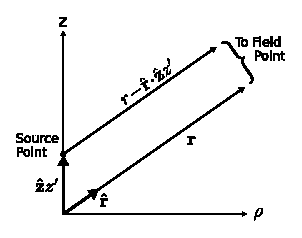
\includegraphics[width=2.5in]{modules/m0198_fParallelRays.eps} 
% https://commons.wikimedia.org/wiki/File:Parallel_ray_approximation_for_an_esd.svg
}}{A rho-z coordinate system. Vector small r starts at the origin and points towards a field point in the positive z and positive rho direction. A short vector boldface small r hat overlays the small r vector. A third vector originates at the origin and goes in the positive z direction to a source point. It is a length boldface small z hat times z prime. A fourth vector originates at the source point and stretches towards the field point. It runs parallel to the small r vector. }
\end{center}
\centerline{\scriptsize 
\copyright~\hyperref[m0198_fParallelRays_Credit]{C.\ Wang} 
\href{https://creativecommons.org/licenses/by-sa/4.0/}{CC BY-SA 4.0} 
} % \centerline 
\caption{
\label{m0198_fParallelRays}
Parallel ray approximation for an ESD.
}
\end{figure}
%
Since we have already assumed that $r\gg L$ (i.e., the distance to field points is much greater than the length of the dipole), the vector ${\bf r}$ is approximately parallel to the vector ${\bf r}-\hat{\bf z}z'$.
Subsequently, it must be true that
%
\begin{equation}
\left|{\bf r}-\hat{\bf z}z'\right| \approx r-\hat{\bf r}\cdot\hat{\bf z}z'
\label{m0198_ePRA}
\end{equation}
%
Note that the magnitude of $r-\hat{\bf r}\cdot\hat{\bf z}z'$ must be approximately equal to $r$, since $r\gg L$.
So, insofar as $\left|{\bf r}-\hat{\bf z}z'\right|$ determines the \emph{magnitude} of $\widetilde{\bf E}({\bf r})$, we may use the approximation:
%
\begin{equation}
\left|{\bf r}-\hat{\bf z}z'\right| \approx r ~~~\mbox{(magnitude)}
\end{equation}
%
Insofar as $\left|{\bf r}-\hat{\bf z}z'\right|$ determines \emph{phase}, we have to be a bit more careful.
The part of the integrand of Equation~\ref{m0198_eE1} that exhibits varying phase is $e^{-j\beta \left|{\bf r}-\hat{\bf z}z'\right|}$.
Using Equation~\ref{m0198_ePRA}, we find
%
\begin{equation}
e^{-j\beta\left|{\bf r}-\hat{\bf z}z'\right|} \approx e^{-j\beta r} e^{+j\beta\hat{\bf r}\cdot\hat{\bf z}z'}
\end{equation}
%
The worst case in terms of phase variation within the integral is for field points along the $z$ axis.
For these points, $\hat{\bf r}\cdot\hat{\bf z}=\pm 1$ and subsequently $\left|{\bf r}-\hat{\bf z}z'\right|$ varies from 
$z-L/2$ to $z+L/2$ where $z$ is the location of the field point.
However, since $L\ll\lambda$ (i.e., because the dipole is electrically short), this difference in lengths is much less than $\lambda/2$.
Therefore, the phase $\beta \hat{\bf r}\cdot\hat{\bf z}z'$ varies by much less than $\pi$ radians, and subsequently $e^{-j\beta\hat{\bf r}\cdot\hat{\bf z}z'}\approx 1$. 
We conclude that under these conditions, 
%
\begin{equation}
e^{-j\beta \left|{\bf r}-\hat{\bf z}z'\right|} \approx e^{-j\beta r} ~~~\mbox{(phase)}
\end{equation}
%
Applying these simplifications for magnitude and phase to Equation~\ref{m0198_eE1}, we obtain:
%
\begin{equation}
\widetilde{\bf E}({\bf r}) \approx \hat{\bf \theta} j \frac{\eta\beta}{4\pi} \left(\sin\theta\right) \frac{e^{-j\beta r}}{r}~\int_{-L/2}^{+L/2} \widetilde{I}(z') dz'
\end{equation}
%
The integral in this equation is very easy to evaluate; in fact, from inspection (Figure~\ref{m0198_fESD}), we determine it is equal to $I_0L/2$.  
Finally, we obtain:
%
\begin{equation}
\boxed{
\widetilde{\bf E}({\bf r}) \approx  \hat{\bf \theta} j \eta \frac{I_0\cdot\beta L}{8\pi} ~\left(\sin\theta\right) ~\frac{e^{-j\beta r}}{r}
}
\label{m0198_eESDE}
\end{equation}
%
Summarizing:
%
%%%%%%%%%%%%%%%%%%%%%%%%%%%%%%%%%%%%%%%%%%%%%%%
%ORB HIGHLIGHT
\begin{mdframed}[backgroundcolor=yellow!20,nobreak=true] 
The electric field intensity radiated by an ESD located at the origin and aligned along the $z$ axis is given by Equation~\ref{m0198_eESDE}.
This expression is valid for $r\gg\lambda$.
\end{mdframed}
%%%%%%%%%%%%%%%%%%%%%%%%%%%%%%%%%%%%%%%%%%%%%%%

It is worth noting that the variation in magnitude, phase, and polarization of the ESD with field point location 
%${\bf r}$ 
is identical to that of a single Hertzian dipole having current moment $\hat{\bf z} I_0 L/2$ (Section~\ref{m0197_Radiation_from_a_Hertzian_Dipole}).
However, the magnitude of the field radiated by the ESD is exactly one-half that of the Hertzian dipole.
Why one-half? Simply because the integral over the triangular current distribution assumed for the ESD is one-half the integral over the uniform current distribution that defines the Hertzian dipole. 
This similarly sometimes causes confusion between Hertzian dipoles and ESDs.  
Remember that ESDs are physically realizable, whereas Hertzian dipoles are not.

It is common to eliminate the factor of $\beta$ in the magnitude using the relationship $\beta=2\pi/\lambda$, yielding:
%
\begin{equation}
\widetilde{\bf E}({\bf r}) \approx  \hat{\bf \theta} j \frac{\eta I_0}{4} \frac{L}{\lambda} ~\left(\sin\theta\right) ~\frac{e^{-j\beta r}}{r}
\end{equation}
%
At field points $r\gg\lambda$, the wave appears to be locally planar.
Therefore, we are justified using the plane wave relationship
\index{plane wave relationships}
$ \widetilde{\bf H} = \frac{1}{\eta} \hat{\bf r} \times \widetilde{\bf E} $
to calculate $\widetilde{\bf H}$.
The result is:
%
\begin{equation}
\widetilde{\bf H}({\bf r}) \approx \hat{\bf \phi} j \frac{I_0}{4} \frac{L}{\lambda} ~\left(\sin\theta\right) ~\frac{e^{-j\beta r}}{r}
\label{m0198_eESDH}
\end{equation}

Finally, let us consider the spatial characteristics of the radiated field.
Figures~\ref{m0198_fEplaneMag} and \ref{m0198_fEplanePol} show the result in a plane of constant $\phi$.
Figures~\ref{m0198_fHplaneMag} and \ref{m0198_fHplanePol} show the result in the $z=0$ plane.
Note that the orientations of the electric and magnetic field vectors indicate a Poynting vector $\widetilde{\bf E}\times\widetilde{\bf H}$ that is always directed radially outward from the location of the dipole.
This confirms that power flow is always directed radially outward from the dipole.
Due to the symmetry of the problem, Figures~\ref{m0198_fEplaneMag}--\ref{m0198_fHplanePol} provide a complete characterization of the relative magnitudes and orientations of the radiated fields.
%
\begin{figure} % <--- "[b!]" for first figure in section *only*; delete for 2nd and subsequent figures
\begin{center}
\pdftooltip{{  % note double braces
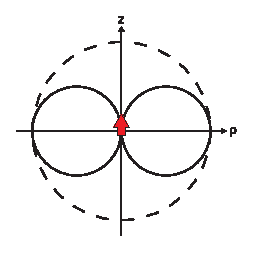
\includegraphics[width=2.5in]{modules/m0198_fEplaneMag.eps} 
% https://commons.wikimedia.org/wiki/File:Magnitude_of_the_Radiated_Field.svg
}}{A rho-z coordinate system has a dashed circle centered at the origin. Two smaller, solid line circles are centered on the rho axis. Each small circle has one edge at the origin and a second edge on the dashed circle. A red arrow pointing up rests on the origin.}
\end{center}
\centerline{\scriptsize 
\copyright~\hyperref[m0198_fEplaneMag_Credit]{S.\ Lally} 
\href{https://creativecommons.org/licenses/by-sa/4.0/}{CC BY-SA 4.0} 
} % \centerline 
\caption{
\label{m0198_fEplaneMag}
Magnitude of the radiated field in any plane of constant $\phi$.
}
\end{figure}
%
\begin{figure} % <--- "[b!]" for first figure in section *only*; delete for 2nd and subsequent figures
\begin{center}
\pdftooltip{{  % note double braces
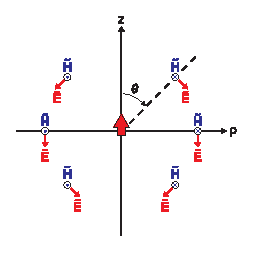
\includegraphics[width=2.5in]{modules/m0198_fEplanePol.eps} 
% https://commons.wikimedia.org/wiki/File:Electric_and_Magnetic_Fields_in_Plane_of_Constant_Theta.svg
}}{There are four points, one in each quadrant, and two points on the rho-axis on either side of the z-axis. At each of the points to the left of the z axis, capital H tilde points out of the page and capital E tilde points counter-clockwise. At each of the points to the right of the z axis, capital H tilde points into the page and capital E tilde points clockwise. Theta is the angle between the z axis and a dotted line running through the point in quadrant 1.
}
\end{center}
\centerline{\scriptsize 
\copyright~\hyperref[m0198_fEplanePol_Credit]{S.\ Lally} 
\href{https://creativecommons.org/licenses/by-sa/4.0/}{CC BY-SA 4.0} 
} % \centerline 
\caption{
\label{m0198_fEplanePol}
Orientation of the electric and magnetic fields in any plane of constant $\phi$.
}
\end{figure}
%
\begin{figure} % <--- "[b!]" for first figure in section *only*; delete for 2nd and subsequent figures
\begin{center}
\pdftooltip{{  % note double braces
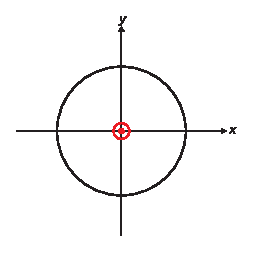
\includegraphics[width=2.5in]{modules/m0198_fHplaneMag.eps} 
% https://commons.wikimedia.org/wiki/File:FHplaneMag.svg
}}{An x-y coordinate system with a circle centered around the origin. A red "out-of-page" symbol at the origin. 
}
\end{center}
\centerline{\scriptsize 
\copyright~\hyperref[m0198_fHplaneMag_Credit]{S.\ Lally} 
\href{https://creativecommons.org/licenses/by-sa/4.0/}{CC BY-SA 4.0} 
} % \centerline 
\caption{
\label{m0198_fHplaneMag}
Magnitude of the radiated field in any plane of constant $z$.
}
\end{figure}
%
\begin{figure} % <--- "[b!]" for first figure in section *only*; delete for 2nd and subsequent figures
\begin{center}
\pdftooltip{{  % note double braces
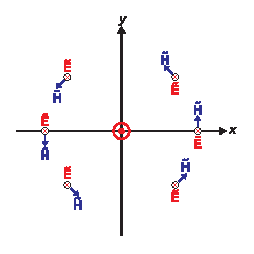
\includegraphics[width=2.5in]{modules/m0198_fHplanePol.eps} 
% https://commons.wikimedia.org/wiki/File:FHplanePol.svg
}}{An x-y coordinate system. A red “out-of-page” symbol at the origin. There are four points, one in each quadrant, and two points on the x-axis on either side of the y-axis. At each of these points, capital H tilde points counter-clockwise and capital E tilde points into the page.}
\end{center}
\centerline{\scriptsize 
\copyright~\hyperref[m0198_fHplanePol_Credit]{S.\ Lally} 
\href{https://creativecommons.org/licenses/by-sa/4.0/}{CC BY-SA 4.0} 
} % \centerline 
\caption{
\label{m0198_fHplanePol}
Orientation of the electric and magnetic fields in the $z=0$ plane.
}
\end{figure}

\index{antenna!electrically-short dipole (ESD)|)}


